\section{Base di dati sistema anagrafe}\label{sec:sbd-sistema-anagrafe}

\subsection{Abstract}

L'obiettivo è sviluppare un servizio che tenga ordinati e renda sempre disponibili tutte le informazioni relative a nomi, gruppi, peculiarità di ognuno dei sensori, delle aree, e dei lampioni. 

Queste informazioni sono particolarmente utili per contestualizzare ognuna delle componenti {\it{hardware}} del sistema.

\subsection{Analisi dei requisiti}

\subsubsection{Descrizione testuale}

Il microservizio di anagrafe ha bisogno di memorizzare, per poter funzionare correttamente, i seguenti dati:

\begin{itemize}
    \item le aree, in particolare le informazioni;
    \item i lampioni e le loro informazioni, ovvero posizione e consumo energetico;
    \item i sensori e le loro informazioni, ovvero posizione e raggio d'azione.
\end{itemize}

Inoltre per i misuratori, ovvero lampioni e sensori, viene salvata anche l'area di appartenenza.

\subsubsection{Glossario dei termini}

Per evitare ambiguità relative alle terminologie utilizzate è stato creato un documento denominato \textit{Glossario}.

Questo documento contiene tutti i termini specifici di settore utilizzati nei documenti, con le relative definizioni.

\subsubsection{Operazioni tipiche}

Le operazioni tipiche che ci si aspetta di avere sono:

\begin{center}
    \begin{tabularx}{\textwidth}{|l|X|}
        \hline
        \rowcolor{gray!30}
        \multicolumn{2}{|c|}{\textbf{OPERAZIONI TIPICHE}}
        \\
        \hline
        \rowcolor{gray!30}
        \textbf{{DESCRIZIONE}} & \textbf{{FREQUENZA D'USO}} \\
        \hline
        Quanti lampioni si trovano all'interno di un'area & Poche volte \\
        \hline
        Quali lampioni si trovano all'interno di un'area & Molte volte\\
        \hline
        Il sensore X che lampioni controlla? & Molte volte \\
        \hline
        Aggiunta di un'area & Poche volte\\
        \hline
        Aggiunta di un lampione ad un'area & Medie volte \\
        \hline
        Aggiunta di un sensore ad un'area & Medie volte\\
        \hline
    \end{tabularx}
\end{center}

\subsection{Progettazione concettuale}

\subsubsection{Analisi delle entità}

\textbf{Se non specificato l'attributo è NOT NULL}

%AREA
\begin{center}
    \begin{tabularx}{\textwidth}{|l|l|l|X|}
        \hline
        \rowcolor{gray!30}
        \multicolumn{4}{|c|}{\textbf{AREA}}\\
        \hline
        id & INTEGER & Identifica univocamente un'area all'interno del sistema & Chiave\\
        \hline
        nome & VARCHAR(50) & \multicolumn{2}{l|}{Il nome dell'area} \\
        \hline
        autoMode & BOOLEAN & \multicolumn{2}{l|}{Specifica se l'area viene gestita in modalità automatica o no (manuale)} \\
        \hline
        lvlInf & VARCHAR(50) & \multicolumn{2}{l|}{In area gestita in modalità automatica, questo è il livello di luminosità} \\ & & \multicolumn{2}{l|}{a cui vengono posti i lampioni se non vengono rilevate persone all'interno dell'area} \\
        \hline
        lvlSup & VARCHAR(20) & \multicolumn{2}{l|}{In area gestita in modalità automatica, questo è il livello di luminosità} \\ & & \multicolumn{2}{l|}{a cui vengono posti i lampioni se vengono rilevate persone all'interno dell'area} \\
        \hline
    \end{tabularx}
\end{center}

%MISURATORE
\begin{center}
    \begin{tabularx}{\textwidth}{|l|l|l|X|}
        \hline
        \rowcolor{gray!30}
        \multicolumn{4}{|c|}{\textbf{MISURATORE}}\\
        \hline
        id & SERIAL & Identifica univocamente un misuratore del livello di luminosità & Chiave\\
        \hline
        tipo & VARCHAR(10) & \multicolumn{2}{l|}{La tipologia del misuratore} \\
        \hline
        latitudine & REAL & \multicolumn{2}{l|}{Latitudine delle coordinate geografiche in cui viene posto il misuratore} \\
        \hline
        longitudine & REAL & \multicolumn{2}{l|}{Longitudine delle coordinate geografiche in cui viene posto il misuratore} \\
        \hline
        idArea & INTEGER & Identifica l'area a cui fa riferimento il misuratore & Chiave esterna: Area(id)\\
        \hline
    \end{tabularx}
\end{center}

%SENSORE
\begin{center}
    \begin{tabularx}{\textwidth}{|l|l|X}
        \hline
        \rowcolor{gray!30}
        \multicolumn{3}{|c|}{\textbf{SENSORE}}\\
        \hline
        raggio & INTEGER & Il raggio d'azione entro il quale il sensore è in grado di rilevare persone \\
        \hline
    \end{tabularx}
\end{center}

%LAMPIONE
\begin{center}
    \begin{tabularx}{\textwidth}{|l|l|X|}
        \hline
        \rowcolor{gray!30}
        \multicolumn{3}{|c|}{\textbf{LAMPIONE}}\\
        \hline
        luminosita & INTEGER & Livello di luminosità in cui si trova il lampione \\
        \hline
        wattaggio & INTEGER & Consumo energetico del lampione \\
        \hline
    \end{tabularx}
\end{center}

\subsubsection{Analisi delle relazioni e delle cardinalità}

\begin{itemize}

    \item Area - Misuratore: \textbf{Appartenenza}
    \begin{itemize}
        \item Un misuratore è contenuto in una ed una sola area (1,1);
        \item Un'area contiene da 0 a N misuratori (0,N);
    \end{itemize}
    
\end{itemize}

\subsubsection{Generalizzazioni}

\begin{itemize}
    \item Lampione è generalizzazione totale esclusiva di Misuratore;
    \item Sensore è generalizzazione totale esclusiva di Misuratore;
\end{itemize}

\subsubsection{Schema ER concettuale}

\begin{center}
    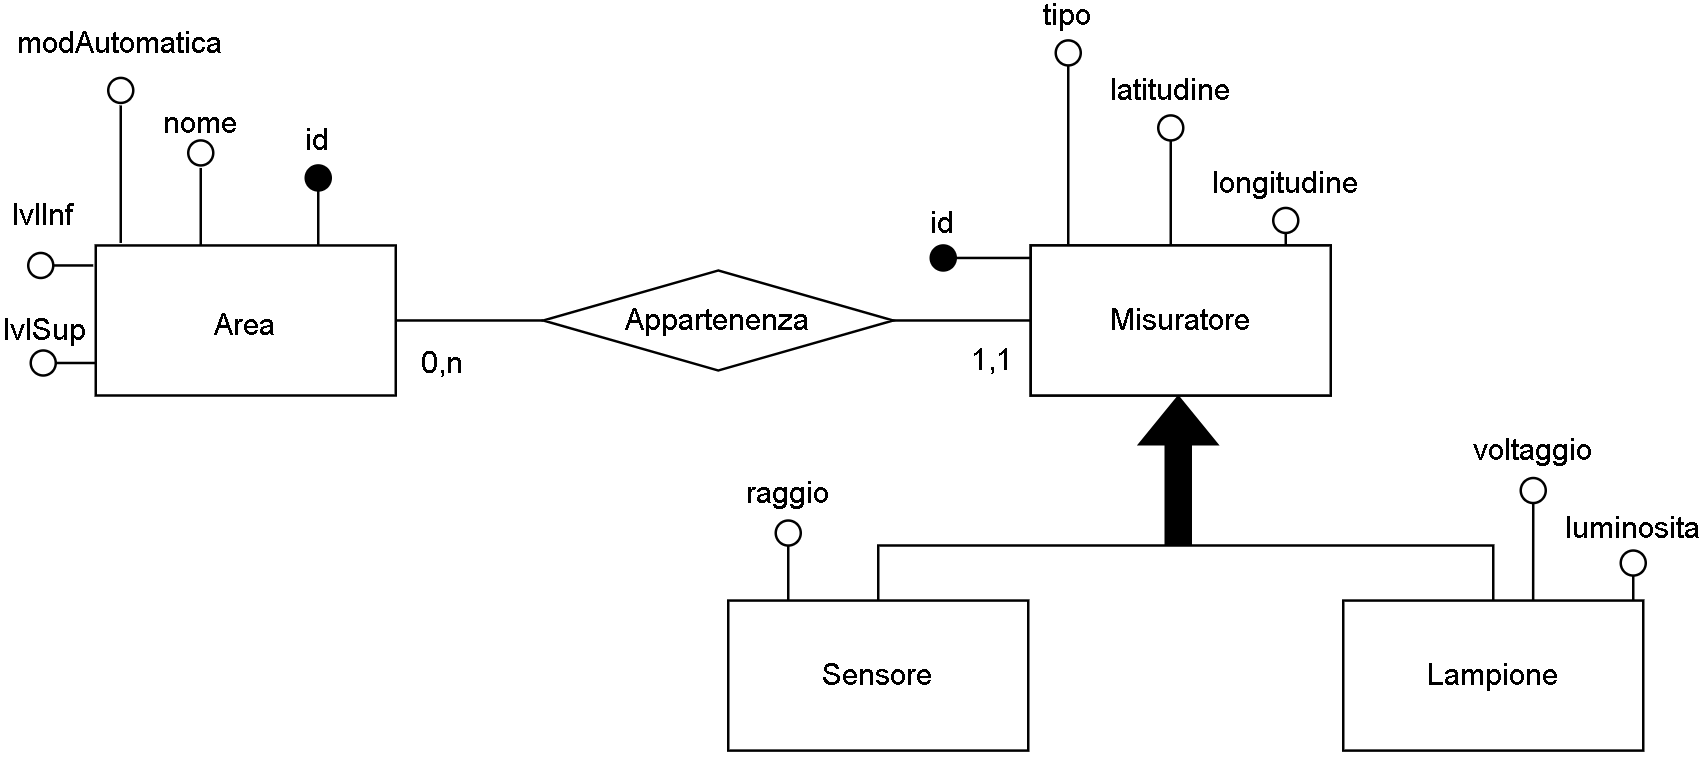
\includegraphics[width=12cm]{contenuti/specifica-basi-dati/img-sbd/anagrafica_concettuale.png}
\end{center}

\subsection{Progettazione logica}

\subsubsection{Eliminazione delle generalizzazioni}

\paragraph{Misuratore}

Per evitare di accorpare le entità Sensore e Lampione nell'entità padre Misuratore, creando così dei campi NULL, è stato deciso di risolvere la generalizzazione mantenendo le tre entità inserendo le relazioni tra le entità figlie e l'entità padre.

\subsubsection{Modifiche, aggiunte e chiarimenti alle chiavi}

Tutte le chiavi primarie sono definite utilizzando le chiavi della progettazione concettuale, tranne nei seguenti casi.

\paragraph{Sensore} Diventando il Sensore un'entità a sé stante, viene aggiunta una chiave esterna, che fungerà anche da chiave primaria, che indica il Misuratore a cui fa riferimento.

\paragraph{Lampione} Diventando il Lampione un'entità a sé stante, viene aggiunta una chiave esterna, che fungerà anche da chiave primaria, che indica il Misuratore a cui fa riferimento.

\subsubsection{Schema concettuale ristrutturato - Schema Logico}

\begin{center}
    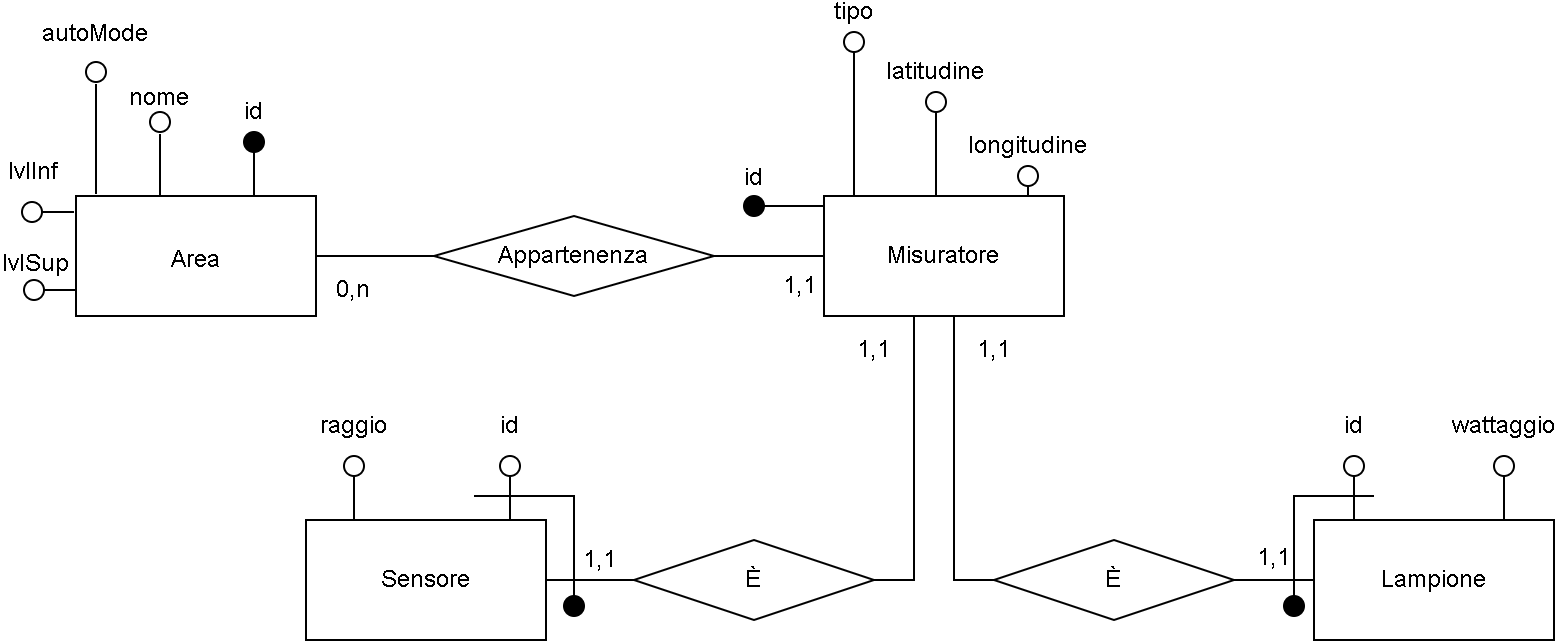
\includegraphics[width=12cm]{contenuti/specifica-basi-dati/img-sbd/anagrafica_logico.png}
\end{center}

\subsubsection{Descrizione schema relazionale}

Per questione di compatibilità con il DBMS alcuni nomi di attributi entità e relazioni sono stati normalizzati, utilizzando il camelCase, togliendo gli accenti, accorciando i nomi molto lunghi e con altre piccole accortezze.
La chiave primaria è indicata in \textbf{grassetto}, le chiavi esterne sono indicate con la \underline{sottolineatura}.

\textit{Area}(\textbf{id}, nome, autoMode, lvlInf, lvlSup) \\
\textit{Misuratore}(\textbf{id}, \underline{idArea}, tipo, latitudine, longitudine) \\
\textit{Sensore}(\underline{\textbf{idMisuratore}}, raggio) \\
\textit{Lampione}(\underline{\textbf{idMisuratore}}, luminosita, wattaggio)

\subsubsection{Vincoli di integrità referenziali}

\textbf{Sensore}.idMisuratore -> \textit{Misuratore}.id \\
\textbf{Lampione}.idMisuratore -> \textit{Misuratore}.id

\subsubsection{Check e constraint}

\paragraph{Area} In \textbf{Area} è attivato un check che controlla che il valore del livello inferiore sia sempre minore del valore del livello superiore.
